
\let\textcircled=\pgftextcircled
\chapter{System design}	\label{chap:design}

\initial{A}s mentioned in Section \ref{sec:methodology}, the design of the Obstacle Collision Avoidance System will follow the Systems Engineering approach.
The main reason is that Systems Engineering provides some methods that prevent the errors with the highest consequences when the system to be designed is complex.
As explained by Rolls-Royce Global Chief of Systems Engineering \cite{beasley2015}:
\begin{quote}
	\itshape
	Systems Engineering collects and organises all the information needed to understand the whole problem, explores it from all angles, and then finds the most appropriate system solution.
\end{quote}

Furthermore, A key study published through INCOSE \cite{incoseuk2016} looked at the phase of detection of errors, and the consequent cost of fixing them.
Cost modelling was validated against a cross-industry range of defence and aerospace projects.
Figure \ref{fig:incose} shows the results of the study.

\begin{figure}[htbp]
	\centering
	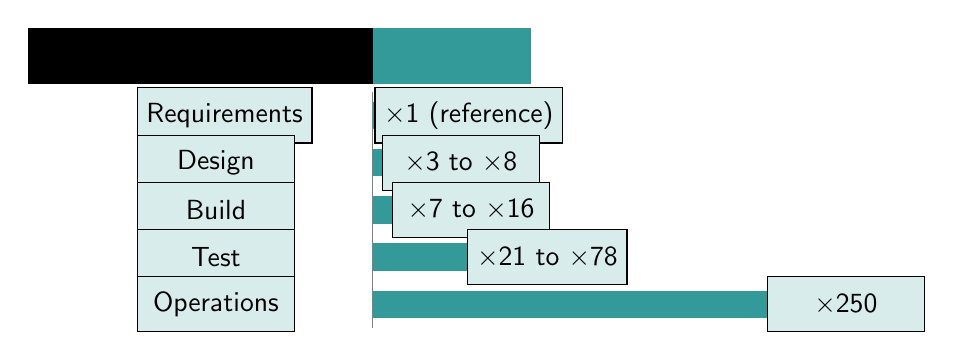
\begin{tikzpicture}

		\colorlet{blueish}{teal!80}

		%\draw[step=1cm,gray,very thin] (0,0) grid (9,6);

		\node[above left,black] at (3,6.2) {\sffamily \large Phase of error detection};
		\node[above right,blueish] at (3,6.2) {\sffamily \bfseries Cost to fix};
		\draw[black!50] (3,6.1) -- (3,3.1);
		\draw[blueish, line width=0.35cm] (3,5.8) -- (3.02,5.8);
			\node[right] at (0,5.8) {\sffamily Requirements};
			\node[right] at (3.02,5.8) {\sffamily $\times$1 (reference)};
		\draw[blueish, line width=0.35cm] (3,5.2) -- (3.11,5.2);
			\node[right] at (0,5.2) {\sffamily Design};
			\node[right] at (3.11,5.2) {\sffamily $\times$3 to $\times$8};
		\draw[blueish, line width=0.35cm] (3,4.6) -- (3.24,4.6);
			\node[right] at (0,4.6) {\sffamily Build};
			\node[right] at (3.24,4.6) {\sffamily $\times$7 to $\times$16};
		\draw[blueish, line width=0.35cm] (3,4) -- (4.2,4);
			\node[right] at (0,4) {\sffamily Test};
			\node[right] at (4.2,4) {\sffamily $\times$21 to $\times$78};
		\draw[blueish, line width=0.35cm] (3,3.4) -- (8,3.4);
			\node[right] at (0,3.4) {\sffamily Operations};
			\node[right] at (8,3.4) {\sffamily $\times$250};

	\end{tikzpicture}
	\caption{Cost to fix a design error. {\footnotesize Source: \cite{incoseuk2016}}}
	\label{fig:incose}
\end{figure}


Hence, in the present chapter, some of the most relevant Systems Engineering tools from the NASA Systems Engineering Handbook \cite{nationalaeronauticsandspaceadministration2007} will be applied


\section{Requirements capture} \label{sec:sysReqs}

The design process for a system is requirement driven, since the requirements are what will define the cost, design, schedule\ldots\ % Space after \ldots
A requirement is a statement about or a characteristic of something that is needed.

Requirements can be derived from a variety of sources, like customer needs, stakeholders, regulations, procedures, constrains, etc.
However, for this project, customers and stakeholders will be disregarded (since none exist) and the motivation as stated in Section \ref{sec:motivation} will be used instead.

In the present section some requirements will be posed, but only those that directly apply to the OCAS subsystem or its interfaces, since the platform is considered to be completely functional prior to the introduction of the solution (following the modularity concept).

%\begin{table}[htbp]
\begin{center}
\begin{longtable}{>{\centering}m{0.7cm}|m{8cm}|>{\centering}m{2.7cm}|>{\centering}m{2.5cm}@{ }c@{ }}

	\hline
	\cellcolor{teal!10}{Req. ID}	&	\centering Requirement	&	Traceability (sourced from)	&	Traceability (allocated to)	&\\ \endfirsthead \endhead

	\hline
	\multicolumn{5}{l}{\cellcolor{black!15}{\footnotesize Certification}} \\
	1.1	&	The UAV shall meet European regulations	&	EC No 218/2008	&	\\
	1.2	&	The UAV shall meet Spanish regulations	&	Ley 18/2014		&	\\

	\hline
	\multicolumn{5}{l}{\cellcolor{black!15}{\footnotesize Architecture}} \\
	2.1	&	The OCAS shall work independently of the UAV	&	Motivation	&	\\
	2.2	&	The OCAS shall be self-contained within the UAV	&	Integration	&	\\

	\hline
	\multicolumn{5}{l}{\cellcolor{black!15}{\footnotesize Functionality}} \\
	3.1	&	The OCAS shall detect obstacles surrounding the UAV	&	Motivation	&	\\
	3.2	&	The OCAS shall avoid collisions with the detected obstacles	&	Motivation	&	\\
	3.3	&	The OCAS shall not interfere with existing Ardupilot functions	&	Motivation	&	\\
	3.4	&	The UAV shall maintain a communications data-link with the GCS at all time	&	Safety / FFBD	&	\\

	\hline
	\multicolumn{5}{l}{\cellcolor{black!15}{\footnotesize Performance}} \\
	4.1	&	The OCAS shall detect obstacles closer than 4 m to the UAV	&	Technical constraint	&	\\
	4.2	&	The OCAS shall detect obstacles of at least 0.5 m across	&	Technical constraint	&	\\
	4.3	&	The OCAS shall be powered along the full mission	&	Safety / FFBD	&	\\

	\hline
	\multicolumn{5}{l}{\cellcolor{black!15}{\footnotesize Interfaces}} \\
	5.1	&	The OCAS shall know the state of the UAV	&	FFBD	&	\\
	5.2	&	The OCAS shall send commands to the UAV	&	FFBD	&	\\
	5.3	&	The OCAS shall be accessible from the GCS	&	Human factors	&	\\
	5.4	&	The OCAS shall be activated and deactivated by the pilot	&	Safety / Human factors	&	\\

	\hline
	\multicolumn{5}{l}{\cellcolor{black!15}{\footnotesize Safety}} \\
	6.1	&	The OCAS shall improve the operational safety of the UAV	&	Motivation	&	\\
	6.2	&	The operation of the OCAS shall not be disrupting to the workflow of the pilot	&	Motivation	&	\\

	\hline
	\multicolumn{5}{l}{\cellcolor{black!15}{\footnotesize Reliability}} \\
	7.1	&	The OCAS shall avoid any physical collision	&	Motivation	&	\\
	7.2	&	The OCAS shall be operative regardless of the state of the controller board	&	Safety	&\\

	\hline
	\multicolumn{5}{l}{\cellcolor{black!15}{\footnotesize Ergonomics and human factors}} \\
	%\multicolumn{5}{l}{} \\
	8.1	&	The OCAS shall be operable after a short training by any pilot	&	Motivation	&	\\
	8.2	&	The OCAS should be engaged and disengaged at discretion of the pilot	&	Safety / FFBD	&	\\ 

	\hline
	\multicolumn{5}{l}{\cellcolor{black!15}{\footnotesize Loads}} \\
	9.1	&	The OCAS shall stand the same loads as the UAV	&	Integration	&	~	&\\

	\hline
	\multicolumn{5}{l}{\cellcolor{black!15}{\footnotesize Weight}} \\
	10.1	&	The UAV + OCAS shall not weight more than the limit of the UAV segment	&	Regulations	&	~	&\\

	\hline
	\multicolumn{5}{l}{\cellcolor{black!15}{\footnotesize Environment}} \\
	11.1	&	The OCAS shall withstand the effect of open-air flight	&	Integration	&	~	&\\

	\hline

	\caption{\cellcolor{white}{System-level requirements}}
	\label{tab:sysReqs}

\end{longtable}

\end{center}
%\end{table}


Notice that Table \ref{tab:sysReqs} is not static, and should be updated during the design process, since some of the tools of Systems Engineering are designed to expose missing requirements.
Thus, some requirements have been written at later design stages, as the ``Traceability (sourced from)'' column shows.
Also, the fourth column is to be completed in the subsystem design stage, when the system requirements will be allocated to one or more specific subsystems or components.


\section{Logical Decomposition}

The Logical Decomposition is an intermediate step between the Requirements Capture and the Design phases.
Its purpose is to understand the manner in which the requirements affect the way that the system functions, for the requirements loop; and to identify a feasible solution that functions in a way that meets the requirements, for the design loop, as shown in Figure \ref{fig:decomposition}


\begin{figure}[htbp]
	\centering
	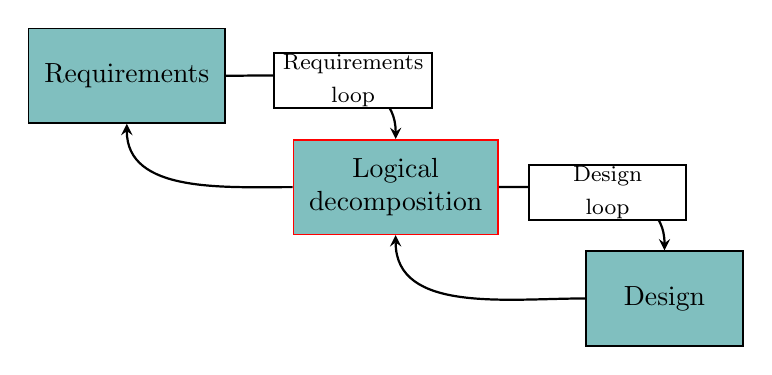
\begin{tikzpicture}
		
		\tikzstyle{function}=[rectangle,
			fill=teal!50,draw=black,semithick,
			minimum height=1.2cm,minimum width=2cm,inner sep=2mm,
			align=center,node distance=2cm]

		\node[function]	(reqs)	{Requirements};
		\node[function,below right of=reqs,xshift=2cm,draw=red]	(logical)	{Logical\\ decomposition};
		\node[function,below right of=logical,xshift=2cm]	(design)	{Design};

		\draw[->,>=stealth,thick,out=0,in=90] (reqs) to node[fill=white,inner sep=-1mm,xshift=2mm,align=center]{\footnotesize Requirements\\\footnotesize  loop} (logical);
		\draw[<-,>=stealth,thick,out=270,in=180] (reqs) to (logical);

		\draw[->,>=stealth,thick,out=0,in=90] (logical) to node[fill=white,inner sep=-1mm,align=center]{\footnotesize Design\\\footnotesize  loop} (design);
		\draw[<-,>=stealth,thick,out=270,in=180] (logical) to (design);

	\end{tikzpicture}
	\caption{The Logical Decomposition phase}
	\label{fig:decomposition}
\end{figure}


\subsection{Functional Architecture}

The logical decomposition performed during the functional analysis decomposes the top level requirements and allocates them down to the lowest desired levels.
The main outcome of the process is the Functional Architecture (Figure \ref{fig:functArch}), which helps establish relationships between requirements, and ultimately build a System Architecture.


\begin{figure}[htpb]
	%\centering
	\hspace{-1cm}
\begin{tikzpicture}

	\tikzstyle{every node}=[rectangle,
		draw=black,fill=teal!20,
		minimum height=0.7cm,minimum width=2cm,
		align=center]
	\tikzstyle{edge from parent}=[black!50,thick,-o,draw]

	\tikzstyle{level 0}=[very thick]
	\tikzstyle{level 1}=[semithick,
		sibling distance=4.5cm,level distance=2.5cm,inner sep=3mm,
		edge from parent fork down]
	\tikzstyle{level 2}=[ultra thin,rounded corners,
		sibling distance=2cm,level distance=1.5cm,inner sep=2mm,
		grow=down,anchor=west,
		edge from parent path={(\tikzparentnode.south west) |- (\tikzchildnode.west)},
		grow via three points={one child at (-3em,-4.5em) and
		two children at (-3em,-4.5em) and (-3em,-7.5em)}]
	
	\node[fill=teal!70]	{\scshape Obstacle Collision Avoidance System}
		child	{node[fill=teal!40] {Communicate with\\ Ground Control}
			child	{node {Create\\ data-link}}
			child	{node {Start OCAS}}
			child	{node {Log information}}
			child	{node {Send information\\ to GCS}}
			child	{node {Stop OCAS}}
		}
		child	{node[fill=teal!40] {Communicate\\ with UAV}
			child	{node {Create\\ data-link}}
			child	{node {Read state}}
			child	{node {Send commands}}
		}
		child	{node[fill=teal!40] {Detect obstacle}
			child	{node {Monitor environment}}
			child	{node {Confirm detection}}
			child	{node {Determine distance}}
			child	{node {Determine velocity}}
			child	{node {Establish level of threat}}
			child	{node {Decide on action}}
		}
		child	{node[fill=teal!40] {Avoid collision}
			child	{node {Compute trajectory}}
			child	{node {Determine\\ recquired actuation}}
			child	{node {Command actuation}}
		};


\end{tikzpicture}

	\caption{OCAS Functional Architecture}
	\label{fig:functArch}

\end{figure}


The main purpose is to create an association between the requirements and the functions that the system needs to be able to perform to meet them.
In the process, any discrepancy or missing items can (and should) be identified and corrected in an iterative manner.

\subsection{Functional Flow Block Diagram (FFBD)}

Once the functions of the system are defined, it is useful to dispose them so that the sequential use of each of them during the mission is shown.
To that end, the Functional Flow Block Diagram is used.
In the FFBD each function is represented by a block, and it is described in terms of inputs, outputs and interfaces.
In the case that a function is composed of several sub-functions, those will be represented hierarchicallyfrom the top level down to the most specific sub-function, maintaining the general flow.

The FFBD shows \emph{what} must happen, and provides an end-to-end path considering all the functionality of the system and the predefined use-case scenarios.
Parallel or alternate paths might be considered.


\begin{figure}[htbp]
\centering
	\begin{tikzpicture}
		
		\tikzstyle{reference}=[ellipse,
			fill=black!30,draw=black,thin,
			minimum height=0.7cm,minimum width=2cm,inner sep=1mm,
			align=center,node distance=3.5cm]
		\tikzstyle{function}=[rectangle,rounded corners,
			fill=teal!40,draw=black,semithick,
			minimum height=0.7cm,minimum width=2cm,inner sep=2mm,
			align=center,node distance=3cm]
		\tikzstyle{logic}=[circle,
			fill=teal!70!black!70,text=white,
			inner sep=1mm,node distance=2cm]
		\tikzstyle{boundary}=[rounded corners,
			draw=red!70!black!100,very thick,dashed]
		\tikzstyle{arrow}=[>=stealth,->,thick]


		\node[function]	(prelaunch)	{1.0/ Pre-launch\\ stage};
		\node[function,right of=prelaunch]	(start-mission)	{2.0/ Start\\ mission};
		\node[logic,right of=start-mission]	(start-and)	{and};
		\node[function,above right of=start-and]	(detect)	{3.0/ Detect\\ obstacle};
		\node[function,right of=detect]	(avoid)	{4.0/ Avoid\\ collision};
		\node[function,right of=start-and,xshift=2cm]	(UAV)	{5.0/ Communicate\\ with UAV};
		\node[function,below right of=start-and]	(GCS)	{6.0/ Communicate\\ with GCS};
		\node[function,below of=start-mission,yshift=-0.5cm]	(power)	{7.0/ Provide\\ power};
		\node[function,right of=UAV,xshift=1.5cm]	(end-mission)	{8.0/ Terminate\\ mission};
		\coordinate[left of=end-mission,node distance=2cm] (end-node) {};

		\draw[arrow] (prelaunch) -- (start-mission);
		\draw[arrow] (start-mission) -- (start-and);
		\draw[arrow] (start-and) |- (detect);
		\draw[arrow] (start-and) -- (UAV);
		\draw[arrow] (start-and) |- (GCS);
		\draw[arrow] (detect) -- (avoid);
		\draw[arrow] (avoid) -| (end-node) -- (end-mission);
		\draw[arrow] (UAV) -- (end-mission);
		\draw[arrow] (GCS) -| (end-node) -- (end-mission);
		\draw[arrow] (prelaunch) |- (power);
		\draw[arrow] (power) -| (end-mission);
		\draw[arrow,dashed] (detect) -- (GCS);
		\draw[arrow,dashed] (UAV) -- (avoid);

		\draw[boundary] ($(prelaunch)+(-1.8cm,-4.5cm)$) -- ($(prelaunch)+(-1.8cm,1cm)$)
			-- ($(prelaunch)+(1.8cm,1cm)$) -- ($(prelaunch)+(1.8cm,-0.8cm)$)
			-- ($(start-and)+(-0.7cm,-0.8cm)$) -- ($(start-and)+(-0.7cm,3cm)$)
			-- ($(end-node)+(0.3cm,3cm)$) -- ($(end-node)+(0.3cm,-4.5cm)$)
			-- cycle;
		
	\end{tikzpicture}

	\caption{OCAS Functional Flow Block Diagram. TOP LEVEL}
	\label{fig:ffbd0}

\end{figure}


\begin{figure}[htbp]
\centering
	\begin{tikzpicture}
		
		\tikzstyle{reference}=[rectangle,rounded corners=0.5cm,
			fill=black!30,draw=black,thin,
			minimum height=0.7cm,minimum width=2cm,inner sep=2mm,
			align=center,node distance=3.5cm]
		\tikzstyle{function}=[rectangle,rounded corners,
			fill=teal!40,draw=black,semithick,
			minimum height=0.7cm,minimum width=2cm,inner sep=2mm,
			align=center,node distance=3.5cm]
		\tikzstyle{logic}=[circle,
			fill=teal!70!black!70,text=white,
			inner sep=1mm,node distance=2cm]
		\tikzstyle{boundary}=[rounded corners,
			draw=red!70!black!100,very thick,dashed]
		\tikzstyle{arrow}=[>=stealth,->,thick]

		\node[reference]	(pilot)	{Ref./\\ Pilot input};
		\node[function,right of=pilot]	(GCS)	{1.1/ Create\\ data-link\\ with GCS};
		\node[function,right of=GCS]	(OCAS)	{1.2/ Start\\ OCAS};
		\node[function,right of=OCAS]	(UAV)	{1.3/ Create\\ data-link\\ with UAV};
		\node[reference,right of=UAV]	(start)	{Ref. 2.0/\\ Start mission};

		\draw[arrow] (pilot) -- (GCS);
		\draw[arrow] (GCS) -- (OCAS);
		\draw[arrow] (OCAS) -- (UAV);
		\draw[arrow] (UAV) -- (start);

		\draw[boundary]	($(GCS)+(-1.5cm,-1.2cm)$) -- ($(GCS)+(-1.5cm,1.2cm)$)
			-- ($(UAV)+(1.5cm,1.2cm)$) -- ($(UAV)+(1.5cm,-1.2cm)$)
			-- cycle;
		
	\end{tikzpicture}

	\caption{OCAS Functional Flow Block Diagram. 1$^{\text{st}}$ STAGE}
	\label{fig:ffbd1}

\end{figure}


\begin{figure}[htbp]
\centering
	\begin{tikzpicture}
		
		\tikzstyle{reference}=[rectangle,rounded corners=0.5cm,
			fill=black!30,draw=black,thin,
			minimum height=0.7cm,minimum width=2cm,inner sep=2mm,
			align=center,node distance=3.5cm]
		\tikzstyle{function}=[rectangle,rounded corners,
			fill=teal!40,draw=black,semithick,
			minimum height=0.7cm,minimum width=2cm,inner sep=2mm,
			align=center,node distance=3cm]
		\tikzstyle{logic}=[circle,
			fill=teal!70!black!70,text=white,
			inner sep=1mm,node distance=2.3cm]
		\tikzstyle{boundary}=[rounded corners,
			draw=red!70!black!100,very thick,dashed]
		\tikzstyle{arrow}=[>=stealth,->,thick]

		\node[reference]	(start)	{Ref. 2.0/\\ Start mission};
		\node[function,below of=start]	(monitor)	{3.1/ Monitor\\ environment};
		\node[reference,below of=monitor]	(GCS)	{Ref. 6.0/\\ Communicate\\ with GCS};
		\node[function,right of=monitor]	(detect)	{3.2/ Confirm\\ detection};
		\node[logic,right of=detect]	(and)	{and};
		\node[function,above right of=and,yshift=-1cm]	(distance)	{3.3/ Evaluate\\ distance};
		\node[function,below right of=and,yshift=1cm]	(velocity)	{3.4/ Evaluate\\ velocity};
		\coordinate[right of=and,xshift=3cm] (coord) {};
		\node[function,right of=coord,xshift=-1.2cm]	(threat)	{3.5/ Evaluate\\ level of threat};
		\node[function,right of=threat]	(decide)	{3.6/ Decide\\ on action};
		\node[reference,below of=decide]	(avoid)	{Ref. 4.0/\\ Avoid collision};

		\draw[arrow] (start) -- (monitor);
		\draw[arrow] (monitor) -- (detect);
		\draw[arrow] (detect) -- (and);
		\draw[arrow] (and) |- (distance);
		\draw[arrow] (and) |- (velocity);
		\draw[arrow] (distance) -| (coord) -- (threat);
		\draw[arrow] (velocity) -| (coord) -- (threat);
		\draw[arrow] (threat) -- (decide);
		\draw[arrow] (decide) -- node[right]{Unsafe}(avoid);
		\draw[arrow] (decide) -- node[right,align=left]{Safe} ($(decide)+(0,1.9cm)$) 
			-- ($(monitor)+(0.3cm,1.9cm)$) -- ($(monitor)+(0.3cm,0.582cm)$);
		\draw[arrow,dashed] (monitor) -- (GCS);

		\draw[boundary] ($(monitor)+(-1.7cm,2.2cm)$) rectangle ($(decide)+(2.2cm,-2.2cm)$);
		
	\end{tikzpicture}

	\caption{OCAS Functional Flow Block Diagram. 3$^{\text{rd}}$ STAGE}
	\label{fig:ffbd3}

\end{figure}


\begin{figure}[htbp]
\centering
	\begin{tikzpicture}
		
		\tikzstyle{reference}=[rectangle,rounded corners=0.5cm,
			fill=black!30,draw=black,thin,
			minimum height=0.7cm,minimum width=2cm,inner sep=2mm,
			align=center,node distance=3.5cm]
		\tikzstyle{function}=[rectangle,rounded corners,
			fill=teal!40,draw=black,semithick,
			minimum height=0.7cm,minimum width=2cm,inner sep=2mm,
			align=center,node distance=3.5cm]
		\tikzstyle{logic}=[circle,
			fill=teal!70!black!70,text=white,
			inner sep=1mm,node distance=2.3cm]
		\tikzstyle{boundary}=[rounded corners,
			draw=red!70!black!100,very thick,dashed]
		\tikzstyle{arrow}=[>=stealth,->,thick]

		\node[reference]	(detect)	{Ref. 3.0/\\ Detect obstacle};
		\node[function,right of=detect]	(trajectory)	{4.1/ Compute\\ trajectory};
		\node[function,right of=trajectory]	(actuation)	{4.2/ Determine\\ actuation};
		\node[function,right of=actuation]	(command)	{4.3/ Command\\ actuation};
		\node[reference,right of=command]	(terminate)	{Ref. 7.0/\\ Terminate\\ mission};
		\node[reference,below of=command,yshift=1.2cm]	(UAV)	{Ref. 5.2/\\ Communicate\\ with UAV};

		\draw[arrow] (detect) -- (trajectory);
		\draw[arrow] (trajectory) -- (actuation);
		\draw[arrow] (actuation) -- (command);
		\draw[arrow] (command) -- (terminate);
		\draw[arrow,dashed] (command) -- (UAV);

		\draw[boundary] ($(trajectory)+(-1.7cm,1cm)$) rectangle ($(command)+(1.8cm,-1cm)$);
		
	\end{tikzpicture}

	\caption{OCAS Functional Flow Block Diagram. 4$^{\text{th}}$ STAGE}
	\label{fig:ffbd4}

\end{figure}


\begin{figure}[htbp]
\centering
	\begin{tikzpicture}
		
		\tikzstyle{reference}=[rectangle,rounded corners=0.5cm,
			fill=black!30,draw=black,thin,
			minimum height=0.7cm,minimum width=2cm,inner sep=2mm,
			align=center,node distance=2.3cm]
		\tikzstyle{function}=[rectangle,rounded corners,
			fill=teal!40,draw=black,semithick,
			minimum height=0.7cm,minimum width=2cm,inner sep=2mm,
			align=center,node distance=3cm]
		\tikzstyle{logic}=[circle,
			fill=teal!70!black!70,text=white,
			inner sep=1mm,node distance=2.5cm]
		\tikzstyle{boundary}=[rounded corners,
			draw=red!70!black!100,very thick,dashed]
		\tikzstyle{arrow}=[>=stealth,->,thick]

		\node[reference]	(start)	{Ref. 2.0/\\ Start mission};
		\node[logic,right of=start]	(and)	{and};
		\node[function,above right of=and,yshift=-1cm]	(read)	{5.1/ Read\\ state};
		\node[function,below right of=and,yshift=1cm]	(send)	{5.2/ Send\\ command};
		\node[reference,below of=send,yshift=0.5cm]	(avoid)	{Ref. 4.3/\\ Avoid collision};
		\coordinate[right of=and,xshift=3cm]	(coord)	{};
		\node[reference,right of=coord]	(terminate)	{Ref. 8.0/\\ Terminate\\ mission};

		\draw[arrow] (start) -- (and);
		\draw[arrow] (and) |- (read);
		\draw[arrow] (and) |- (send);
		\draw[arrow,dashed] (avoid) -- (send);
		\draw[arrow] (read) -| (coord) -- (terminate);
		\draw[arrow] (send) -| (coord) -- (terminate);

		\draw[boundary] ($(and)+(-0.8cm,2cm)$) rectangle ($(coord)+(0.8cm,-2cm)$);
		
	\end{tikzpicture}

	\caption{OCAS Functional Flow Block Diagram. 5$^{\text{th}}$ STAGE}
	\label{fig:ffbd5}

\end{figure}


\begin{figure}[htbp]
\centering
	\begin{tikzpicture}
		
		\tikzstyle{reference}=[rectangle,rounded corners=0.5cm,
			fill=black!30,draw=black,thin,
			minimum height=0.7cm,minimum width=2cm,inner sep=2mm,
			align=center,node distance=3cm]
		\tikzstyle{function}=[rectangle,rounded corners,
			fill=teal!40,draw=black,semithick,
			minimum height=0.7cm,minimum width=2cm,inner sep=2mm,
			align=center,node distance=3cm]
		\tikzstyle{logic}=[circle,
			fill=teal!70!black!70,text=white,
			inner sep=1mm,node distance=2.5cm]
		\tikzstyle{boundary}=[rounded corners,
			draw=red!70!black!100,very thick,dashed]
		\tikzstyle{arrow}=[>=stealth,->,thick]

		\node[reference]	(start)	{Ref. 2.0/\\ Start mission};
		\node[reference,below of=start,yshift=1cm]	(detect)	{Ref. 3.1/\\ Detect obstacle};
		\node[function,right of=start]	(GCS)	{6.1/ Send\\ information\\ to GCS};
		\node[function,right of=GCS]	(log)	{6.2/ Log\\ information};
		\node[reference,right of=log]	(terminate)	{Ref. 8.0/\\ Terminate\\ mission};

		\draw[arrow] (start) -- (GCS);
		\draw[arrow] (GCS) -- (log);
		\draw[arrow] (log) -- (terminate);
		\draw[arrow,dashed] (detect) -| (GCS);

		\draw[boundary] ($(GCS)+(-1.5cm,1.2cm)$) rectangle ($(log)+(1.5cm,-1.2cm)$);
		
	\end{tikzpicture}

	\caption{OCAS Functional Flow Block Diagram. 6$^{\text{th}}$ STAGE}
	\label{fig:ffbd6}

\end{figure}




For the block diagrams depicted in Figures \ref{fig:ffbd0} to \ref{fig:ffbd6}, the symbology explained below is used:

\begin{itemize}
	\item 
		\tikz \draw[rounded corners=1mm,fill=teal!40,draw=black,semithick] (0,0) rectangle (6mm,3mm);
		\ represents an individual function or subfunction as defined in the Functional Architecture from Figure \ref{fig:functArch}.
	\item
		\tikz \draw[circle,fill=teal!70!black!70,draw=none,text=white,inner sep=1mm,node distance=2cm] (0,0) circle (2mm);
		\ represents a logical \textit{and} or \textit{or} gate for defining parallel or alternative paths, respectively.
	\item
		\tikz \draw[rectangle,rounded corners=1.5mm,fill=black!30,draw=black,thin] (0,0) rectangle (5mm,3mm);
		\ represents a reference block that specifies the origin or destination of a path from an external function of the system.
	\item
		\tikz \draw[rounded corners=1mm,draw=red!70!black!100,very thick,dashed] (0,0) rectangle (6mm,3mm);
		\ represents the boundaries of the functional description, be it the whole system or a subfunction of it.
	\item
		\tikz \draw[>=stealth,->,thick] (0,0) -- (5mm,0);
		\ indicates the secuential order that is to be followed from one function to another.
	\item
		\tikz \draw[>=stealth,->,thick,dashed] (0,0) -- (5mm,0);
		\ indicates an information flow between two functional blocks.
\end{itemize}


\subsection{Product Breakdown Structure (PBS)}

Once the functions are properly defined, they need to be allocated to the subsystems that will be in charge of accomplishing them.
To that end, the system is decomposed in its forming subsystems ensuring that all the functions can be achieved by the system.
The decomposition process is visually show via the Product Breakdown Structure, which is represented in Figure \ref{fig:pbs}

\begin{figure}[htbp]
	\centering
	\begin{tikzpicture}
		
		\tikzstyle{every node}=[rectangle,
			draw=black,fill=teal!15,
			minimum height=0.7cm,minimum width=2cm,
			align=center]
		\tikzstyle{edge from parent}=[black!50,thick,-o,draw]

		\tikzstyle{level 0}=[very thick]
		\tikzstyle{level 1}=[semithick,
			sibling distance=8cm,level distance=2cm,inner sep=3mm,
			edge from parent fork down]
		\tikzstyle{level 2}=[semithick,
			sibling distance=3cm,level distance=2cm,inner sep=3mm,
			edge from parent fork down]
		\tikzstyle{level 3}=[ultra thin,rounded corners,
			sibling distance=2cm,level distance=1.5cm,inner sep=1mm,
			grow=down,anchor=west,
			edge from parent path={(\tikzparentnode.south west) |- (\tikzchildnode.west)},
			grow via three points={one child at (-2em,-4.5em) and
			two children at (-2em,-4.4em) and (-2em,-7.6em)}]
		
		\node[fill=teal!70]	{\scshape Obstacle Collision Avoidance System}
			child	{node[fill=teal!40] {Hardware}
				child	{node[fill=teal!20] {1.0/ Computer\\ board}
					child	{node {1.1/ Processing\\ unit}}
					child	{node {1.2/ Peripheral\\ connections}}
				}
				child	{node[fill=teal!20] {2.0/ Sensors}}
				child	{node[fill=teal!20] {3.0/ Structure}
					child	{node {3.1/ Sensor\\ mount}}
					child	{node {3.2/ Computer\\ mount}}
				}
				child	{node[fill=teal!20] {4.0/ Power}}
			}
			child	{node[fill=teal!40] {Software}
				child	{node {5.0/ Program\\ driver}
					child	{node {5.1/ GCS\\ connector}}
					child	{node {5.2/ Sensor\\ operator}}
					child	{node {5.3/ Signal\\ processor}}
					child	{node {5.4/ Actuation\\ calculator}}
					child	{node {5.5/ UAV\\ connector}}
				}
			}
		;

	\end{tikzpicture}
	\caption{OCAS Product Breakdown Structure}
	\label{fig:pbs}
\end{figure}



\subsection{Functional-Physical matrix}

Finally, to couple the Requirements (Table \ref{tab:sysReqs}) with the Functional Architecture (Figure \ref{fig:functArch}) and with the Physical product (Figure \ref{fig:pbs}), a functional-physical matrix can be built.
This tool is very relevant since it exposes possible mismatches between the three steps, which would lead to requirements not being met or a product that cannot perform its intended functions.
Thus, by filling the matrix, the designer can go back to previous steps and adjust anything that is needed in order to avoid the exponential increase in cost that was mentioned at the beginning of the present Chapter.

For the matrix represented in Table \ref{tab:functPhys}, the requirements, functions and subsystems have been represented by their ID as defined in Table \ref{tab:sysReqs}, Figures \ref{fig:ffbd0} to \ref{fig:ffbd6} and Figure \ref{fig:pbs}, respectively.

\begin{table}
	\centering
	\begin{tabular}{cccccccc}

	\end{tabular}
	\caption{OCAS Functional-Physical matrix}
	\label{tab:functPhys}
\end{table}


As it can be seen for requirements 9.1, 10.1 and 11.1, they are requirements affecting the entire system, and thus cannot be associated to any function: they are requirements that impose hardware constrains only.

\subsection{Interfaces definition (N$^2$ diagram)} \label{sec:interfaces}

For the correct integration of the system the definition of its interfaces is of utmost importance.
The N$^2$ diagram is commonly used for the development of those interfaces.

In the N$^2$ diagram, an N$\times$N matrix is built.
In the main diagonal all the systems or subsystems are placed, while the upper and lower triangles are reserved for the interfaces, which are clasified into inputs and outputs.
An input to any of the modules is represented through its vertical cells, while the output is place on the horizontal rows.
An example N$^2$ diagram can be found in Figure \ref{fig:N2example}

\begin{figure}[htbp]
	\centering

	\begin{subfigure}[c]{0.3\textwidth}

		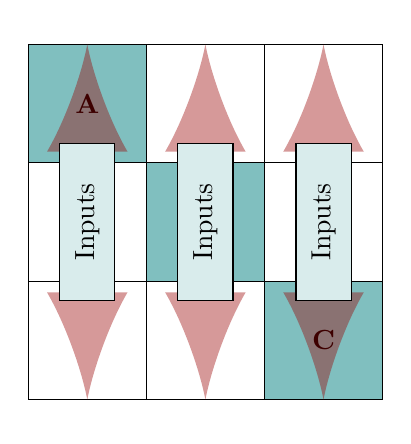
\begin{tikzpicture}

			\tikzstyle{interface}=[fill=white,draw=black,
				minimum width=1.5cm,minimum height=1.5cm,
				node distance=1.5cm]
			\tikzstyle{module}=[fill=teal!50,draw=black,
				minimum width=1.5cm,minimum height=1.5cm,
				node distance=1.5cm,
				align=center]

			\node[module]		(11)	{\bfseries A};
			\node[interface,right of=11]	(12)	{};
			\node[interface,right of=12]	(13)	{};
			\node[interface,below of=11]	(21)	{};
			\node[module,right of=21]		(22)	{\bfseries B};
			\node[interface,right of=22]	(23)	{};
			\node[interface,below of=21]	(31)	{};
			\node[interface,right of=31]	(32)	{};
			\node[module,right of=32]		(33)	{\bfseries C};

			\begin{scope}[transparency group,opacity=0.4]
				\draw[red!60!black,line width=12pt,latex-latex]
					(11.north)  -- (31.south);
				\draw[red!60!black,line width=12pt,latex-latex]
					(12.north)  -- (32.south);
				\draw[red!60!black,line width=12pt,latex-latex]
					(13.north)  -- (33.south);
			\end{scope}
				\node[rotate=90] at (21) {Inputs};
				\node[rotate=90] at (22) {Inputs};
				\node[rotate=90] at (23) {Inputs};
				
			\end{tikzpicture}

		\caption{N$^2$ inputs}
	\end{subfigure}
	\hfill
	\begin{subfigure}[c]{0.3\textwidth}

		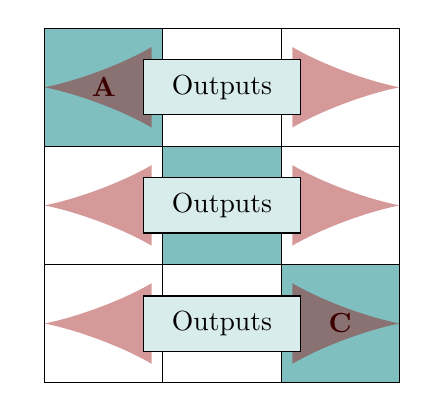
\begin{tikzpicture}
			
			\tikzstyle{interface}=[fill=white,draw=black,
				minimum width=1.5cm,minimum height=1.5cm,
				node distance=1.5cm]
			\tikzstyle{module}=[fill=teal!50,draw=black,
				minimum width=1.5cm,minimum height=1.5cm,
				node distance=1.5cm,
				align=center]

			\node[module]		(11)	{\bfseries A};
			\node[interface,right of=11]	(12)	{};
			\node[interface,right of=12]	(13)	{};
			\node[interface,below of=11]	(21)	{};
			\node[module,right of=21]		(22)	{\bfseries B};
			\node[interface,right of=22]	(23)	{};
			\node[interface,below of=21]	(31)	{};
			\node[interface,right of=31]	(32)	{};
			\node[module,right of=32]		(33)	{\bfseries C};

			\begin{scope}[transparency group,opacity=0.4]
				\draw[red!60!black,line width=12pt,latex-latex]
					(11.west)  -- (13.east);
				\draw[red!60!black,line width=12pt,latex-latex]
					(21.west)  -- (23.east);
				\draw[red!60!black,line width=12pt,latex-latex]
					(31.west)  -- (33.east);
			\end{scope}
				\node at (12){Outputs};
				\node at (22){Outputs};
				\node at (32){Outputs};

		\end{tikzpicture}

		\caption{N$^2$ outputs}
	\end{subfigure}
	\hfill
	\begin{subfigure}[c]{0.3\textwidth}

		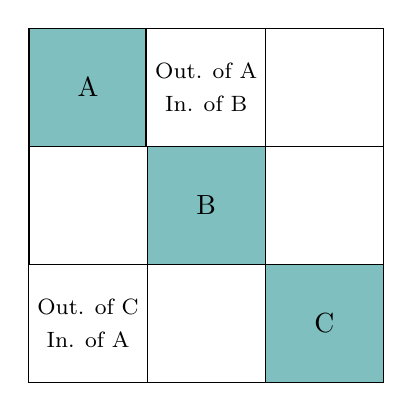
\begin{tikzpicture}
			
			\tikzstyle{interface}=[fill=white,draw=black,
				minimum width=1.5cm,minimum height=1.5cm,
				node distance=1.5cm,
				align=center]
			\tikzstyle{module}=[fill=teal!50,draw=black,
				minimum width=1.5cm,minimum height=1.5cm,
				node distance=1.5cm,
				align=center]

			\node[module]		(11)	{A};
			\node[interface,right of=11]	(12)	{\footnotesize Out. of A\\ \footnotesize In. of B};
			\node[interface,right of=12]	(13)	{};
			\node[interface,below of=11]	(21)	{};
			\node[module,right of=21]		(22)	{B};
			\node[interface,right of=22]	(23)	{};
			\node[interface,below of=21]	(31)	{\footnotesize Out. of C\\ \footnotesize In. of A};
			\node[interface,right of=31]	(32)	{};
			\node[module,right of=32]		(33)	{C};

		\end{tikzpicture}

		\caption{N$^2$ diagram}
	\end{subfigure}

	\caption{Example of a N$^2$ diagram}
	\label{fig:N2example}
\end{figure}



For the Obstacle Collision Avoidance System N$^2$ diagram in Figure \ref{fig:N2}, the subsystems defined in the Product Breakdown Structure (Figure \ref{fig:pbs}) will be placed in the main diagonal.


\begin{figure}[htbp]
	\hspace{-1.9cm}
	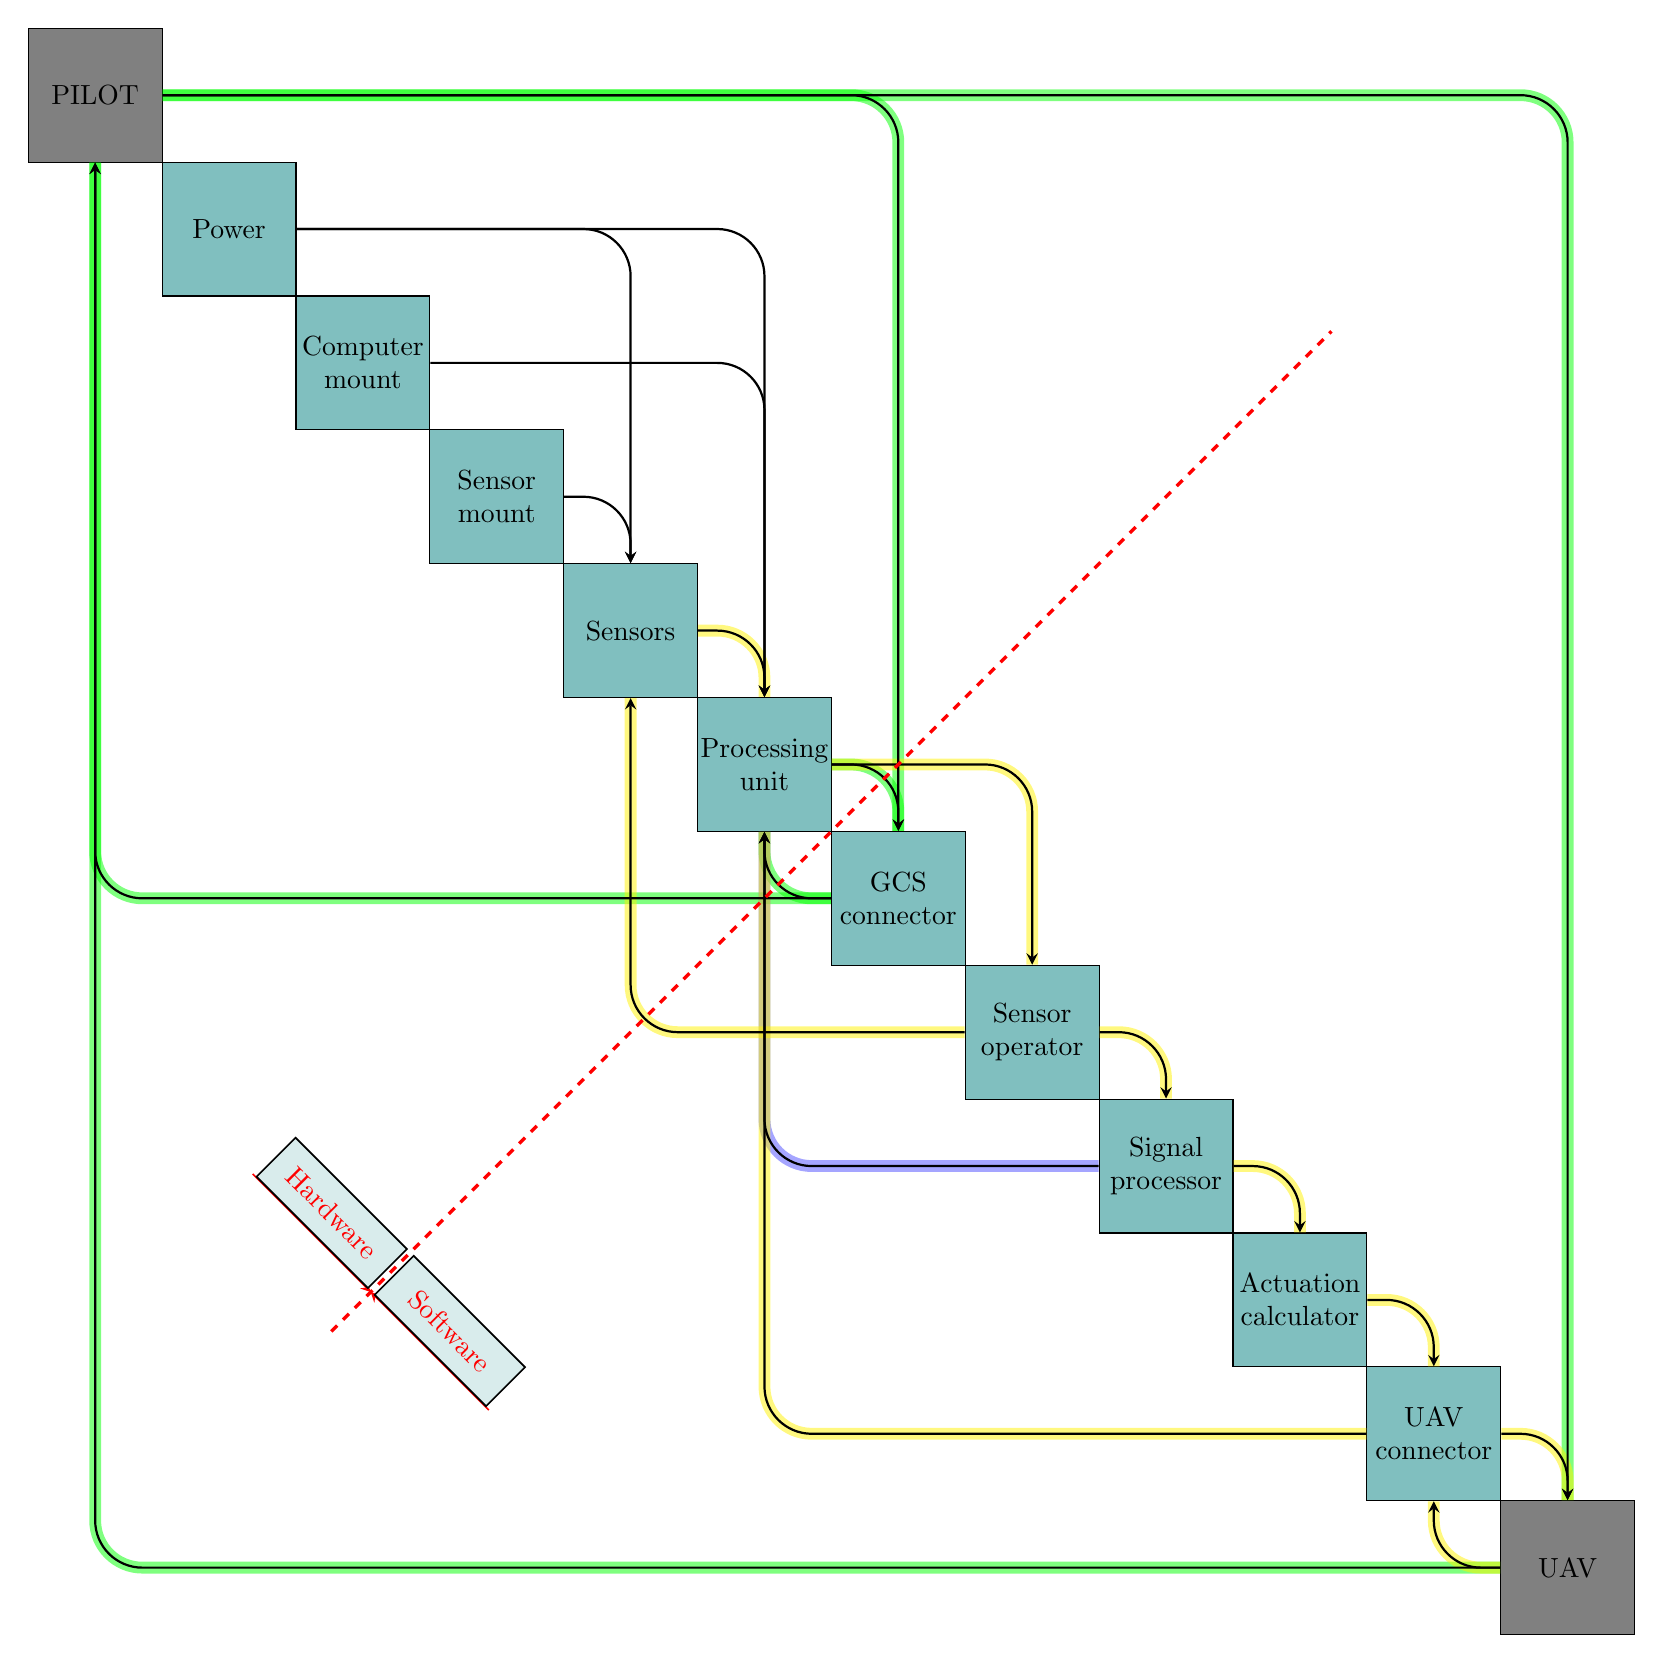
\begin{tikzpicture}

		\tikzstyle{module}=[rectangle,
			fill=teal!50,draw=black,
			minimum height=1.7cm,minimum width=1.7cm,
			node distance=2.4042cm,	%=sqrt(1.7cm)
			align=center,inner sep=0mm]
		\tikzstyle{arrow}=[->,>=stealth,
			draw=black,thick,
			rounded corners=0.6cm]
		\tikzstyle{shadow}=[
			draw=black,opacity=0.5,line width=1.5mm,
			rounded corners=0.6cm]

		\node[module,fill=gray]	(pilot)	{PILOT};
		\node[module,below right of=pilot]	(power)	{Power};
		\node[module,below right of=power]	(computer-m)	{Computer\\ mount};
		\node[module,below right of=computer-m]	(sensor-m)	{Sensor\\ mount};
		\node[module,below right of=sensor-m]	(sensors)	{Sensors};
		\node[module,below right of=sensors]	(cpu)	{Processing\\ unit};
		\node[module,below right of=cpu]	(gcs)	{GCS\\ connector};
		\node[module,below right of=gcs]	(sensor-o)	{Sensor\\ operator};
		\node[module,below right of=sensor-o]	(signal)	{Signal\\ processor};
		\node[module,below right of=signal]	(actuation)	{Actuation\\ calculator};
		\node[module,below right of=actuation]	(uav)	{UAV\\ connector};
		\node[module,below right of=uav,fill=gray]	(UAV)	{UAV};


			\draw[shadow,draw=green]	(pilot)		-|	(gcs);
			\draw[shadow,draw=green]	(pilot)		-|	(UAV);
			\draw[shadow,draw=green]	(UAV)		-|	(pilot);
			\draw[shadow,draw=green]	(gcs)		-|	(pilot);
			\draw[shadow,draw=yellow]	(sensors)	-|	(cpu);
			\draw[shadow,draw=green]	(cpu)		-|	(gcs);
			\draw[shadow,draw=green]	(gcs)		-|	(cpu);
			\draw[shadow,draw=yellow]	(cpu)		-|	(sensor-o);
			\draw[shadow,draw=blue!70]	(signal)		-|	(cpu);
			\draw[shadow,draw=yellow]	(uav)		-|	(cpu);
			\draw[shadow,draw=yellow]	(sensor-o)	-|	(signal);
			\draw[shadow,draw=yellow]	(sensor-o)	-|	(sensors);
			\draw[shadow,draw=yellow]	(signal)	-|	(actuation);
			\draw[shadow,draw=yellow]	(actuation)	-|	(uav);
			\draw[shadow,draw=yellow]	(uav)		-|	(UAV);
			\draw[shadow,draw=yellow]	(UAV)		-|	(uav);
		
		\draw[arrow]	(pilot)		-|	(gcs);
		\draw[arrow]	(pilot)		-|	(UAV);
		\draw[arrow]	(UAV)		-|	(pilot);
		\draw[arrow]	(gcs)		-|	(pilot);

		\draw[arrow]	(power)		-|	(sensors);
		\draw[arrow]	(power)		-|	(cpu);

		\draw[arrow]	(computer-m)-|	(cpu);

		\draw[arrow]	(sensor-m)	-|	(sensors);

		\draw[arrow]	(sensors)	-|	(cpu);

		\draw[arrow]	(cpu)		-|	(gcs);
		\draw[arrow]	(gcs)		-|	(cpu);
		\draw[arrow]	(cpu)		-|	(sensor-o);
		\draw[arrow]	(signal)	-|	(cpu);
		\draw[arrow]	(uav)		-|	(cpu);

		\draw[arrow]	(sensor-o)	-|	(signal);
		\draw[arrow]	(sensor-o)	-|	(sensors);

		\draw[arrow]	(signal)	-|	(actuation);

		\draw[arrow]	(actuation)	-|	(uav);

		\draw[arrow]	(uav)		-|	(UAV);
		\draw[arrow]	(UAV)		-|	(uav);


		\draw[red,very thick,dashed]	(3,-15.7) -- (15.7,-3);
		\draw[red,->,>=stealth,semithick]	(2,-13.7) -- node[sloped,anchor=south]{Hardware} (3.5,-15.2);
		\draw[red,<-,>=stealth,semithick]	(3.5,-15.2) -- node[sloped,anchor=south]{Software} (5,-16.7);

	\end{tikzpicture}

	\caption{OCAS N$^2$ diagram for interfaces definition}
	\label{fig:N2}
\end{figure}


In this Figure, the grey blocks represent external systems to the OCAS, while the blue ones are subsystems of the OCAS itself.
In a regular UAV, with no OCAS implemented, the pilot would only be executing the outermost green loop: only in direct control with the UAV.
Nonetheless, the OCAS provides an additional layer of safety that is functionally placed between the pilot and the UAV; but also adds another interface the pilot has to deal with: the GCS connector is the gate to the OCAS, which in turn connects via the Central Processing Unit to the rest of the system.
Hence, the ``green'' interfaces designate the human links with both the OCAS and the UAV.

Further, the ``yellow'' interfaces have been highlighted since they represent the traditional sensing and control problem.
Notice how the state of the UAV is transmitted from the UAV connector (that information is relayed by the UAV) and the sensors to the Processing Unit.
From the hardware-software interface downwards, the information is processed, the actuation calculated and ultimately the command is sent to the UAV. 

The ``blue'' interface has been created for information logging in response to Function 6.2 as defined in the FFBD.
It could also serve as a debugging channel during the implementation phase.

Finally, the ``black'' interfaces on the hardware side shows how the system has been designed meeting requirements 2.1 and 2.2, which stated that the OCAS shall be independent of the UAV and self-contained.
In this case, it has been decided that the OCAS would carry its own power source to provide energy to its components.
However, the power is not transmitted down to the UAV, which could be more weight efficient but would significantly modify the architecture of the original UAV, disregarding one of the main requirements from the motivation of the project.


\section{Component choice}

Only after properly defining the requirements, functions and subsystems of the Obstacle Collision Avoidance System can the components be chosen to ensure that the system is correctly designed to meet specifications.

\subsection{Sensors}

The most relevant sensing alternatives were already exposed in Section \ref{sec:sensing}.
In this Section, the most appropriate one for the project will be chosen according to the specifications.

Certainly, all the options considered have their advantages and disadvantages.
The purpose of the selection process is to evaluate all of those in a trade-off study which ensures that the final selection provides the best alternative to the system.
The steps to a successful trade-off study are:
\begin{enumerate}
	\item Definition of the problem
	\item Definition of the constraints
	\item Generation of alternative solutions
	\item Definition of the evaluation criteria
	\item Definition of the weight factors
	\item Fulfillment of the trade study
	\item Ranking of the solutions
\end{enumerate}

For the three first steps, those have already been done in Chapter \ref{chap:problem}, Section \ref{sec:sysReqs} and Section \ref{sec:sensing}, respectively.

For the rest of the steps, a tabular format will be used.

The evaluation criteria can be defined as the parameters considered important for the sensors to fulfill towards the correct achievement of their function, and will be presented on the first column of the table.

A weight factor will be given to each of the evaluation criteria according to their importance in the sensing and integration problems.
Those will be normalised ensuring that the sum of all of them add up to unity, and will be presented in the second column of the table.

The trade study will then be fulfilled by rating each of the alternatives on the evaluation criteria as previously defined.
The mark given, ranging from 0 to 1, represents the capability of the alternative on the corresponding evaluation criteria.

Finally, the ranking of the solutions is performed by combining (multiplying) the criteria's weight factors with the ratings given to the alternatives on each of those criteria, to ultimately sum all of those and obtain a single figure for every alternative considered.
The objectively most appropriate alternative is the one with highest rating after the trade-off study.


\begin{table}[htbp]
	\centering
	\begin{tabular}{lc|ll|ll|ll|lcl}
		
		\hline
					&					&	\multicolumn{2}{c|}{Computer vision}&	\multicolumn{2}{c|}{Sonar}	&	\multicolumn{2}{c|}{Lidar}	&	\multicolumn{2}{c}{Radar}	\\
		Criteria	&	Weight factor	&	Rating	&	Combined				&	R	&	C					&	R	&	C					&	R	&	C					\\
		\hline
		Accuracy			&	0.1	&	0.4	&	0.04	&	0.8	&	0.08&	1	&	0.1	&	0.6	&	0.06	\\
		Range				&	0.12&	1	&	0.12	&	0.4	&	0.048&	0.8	&	0.096&	0.6	&	0.072	\\
		Ease of operation	&	0.12&	0.6	&	0.072	&	1	&	0.12&	0.6	&	0.072&	0.4	&	0.048	\\
		Ease of integration	&	0.15&	0.6	&	0.09	&	0.8	&	0.12&	0.6	&	0.09&	0.2	&	0.03	\\
		Ease of processing	&	0.12&	0.2	&	0.024	&	1	&	0.12&	0.8	&	0.096&	0.6	&	0.072	\\
		Availability		&	0.12&	0.8	&	0.096	&	0.8	&	0.096&	0.6	&	0.072&	0.6	&	0.072	\\
		Cost				&	0.1	&	0.6	&	0.06	&	1	&	0.1	&	0.2	&	0.02&	0.8	&	0.08	\\
		Flexibility			&	0.05&	1	&	0.05	&	0.4	&	0.02&	0.4	&	0.02&	0.6	&	0.03	\\
		Weight				&	0.12&	1	&	0.12	&	0.8	&	0.096&	0.4	&	0.048&	0.8	&	0.096	\\
		\hline
		\scshape Total		&		&		&	0.672	&		&\bf 0.8&		&	0.614&		&	0.56	\\

	\end{tabular}
	\caption{Sensor alternatives trade-off study}
	\label{tab:tradeoff}
\end{table}


As it can be seen in Table \ref{tab:tradeoff}, the most appropriate sensor to be used in the OCAS is the ultrasonic rangefinder.
The reasons for that are mainly the high score obtained in the ease of operation, integration and processing, as will be seen during the implementation process, as well as its low cost; which were all considered to be important properties for the chosen sensor to meet for this project.


\begin{figure}[htbp]
	\centering
	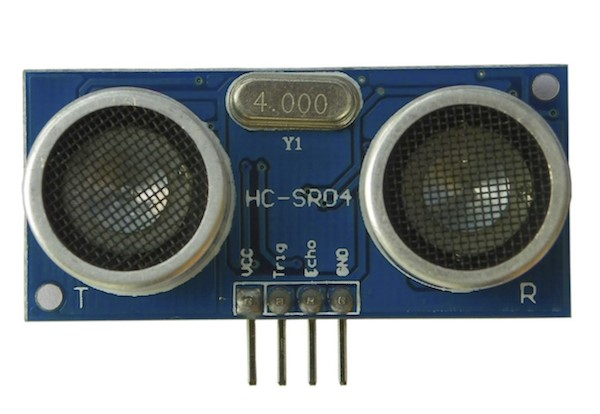
\includegraphics[width=0.3\textwidth]{./figures/hc-sr04.jpg}
	\caption{Chosen ultrasonic rangefinder: HC-SR04 {\footnotesize Source: \url{arduinolearning.com}}}
	\label{fig:hc-sr04}
\end{figure}


\subsection{Computer board}

The choice of processing unit for the OCAS is not nearly as complex as the sensor case.
The main available alternatives are either a microcontroller board or a Single Board Computer (SBC), which differ in the type of CPU architecture.

A microcontroller board can be as simple as a single Atmel AVR microchip, although they generally incorporate additional features for easier programming and connection with other peripherals.
The best example of microcontroller boards is the Arduino family.
These board usually incorporate an 8-bit processing unit, which can be considered computationally underpowered according to present standards, and thus the programs are frequently coded in C/C++ languages due to their high resource efficiency.
Also, these boards do not have any software feature out-of-the-box, which implies that every required function needs to be programmed from scratch on the chip.

On the other hand, an SBC can be thought of as a full Personal Computer, except in a reduced form-factor.
These computers do not generally exceed the footprint of a credit card, albeit embodying all the necessary components such as RAM and non-volatile memory, USB ports and even the convenient General Purpose Input / Output (GPIO) pins for low-level hardware integration.
Moreover, SBCs are driven by complete Operating Systems (OS), featuring convenient general kernel and communications tools.
Additionally, these computers are able to run virtually any computer software available, which also means that applications can be programmed in a wide range of languages. 

\begin{wrapfigure}{r}{0.3\textwidth}
	\centering
	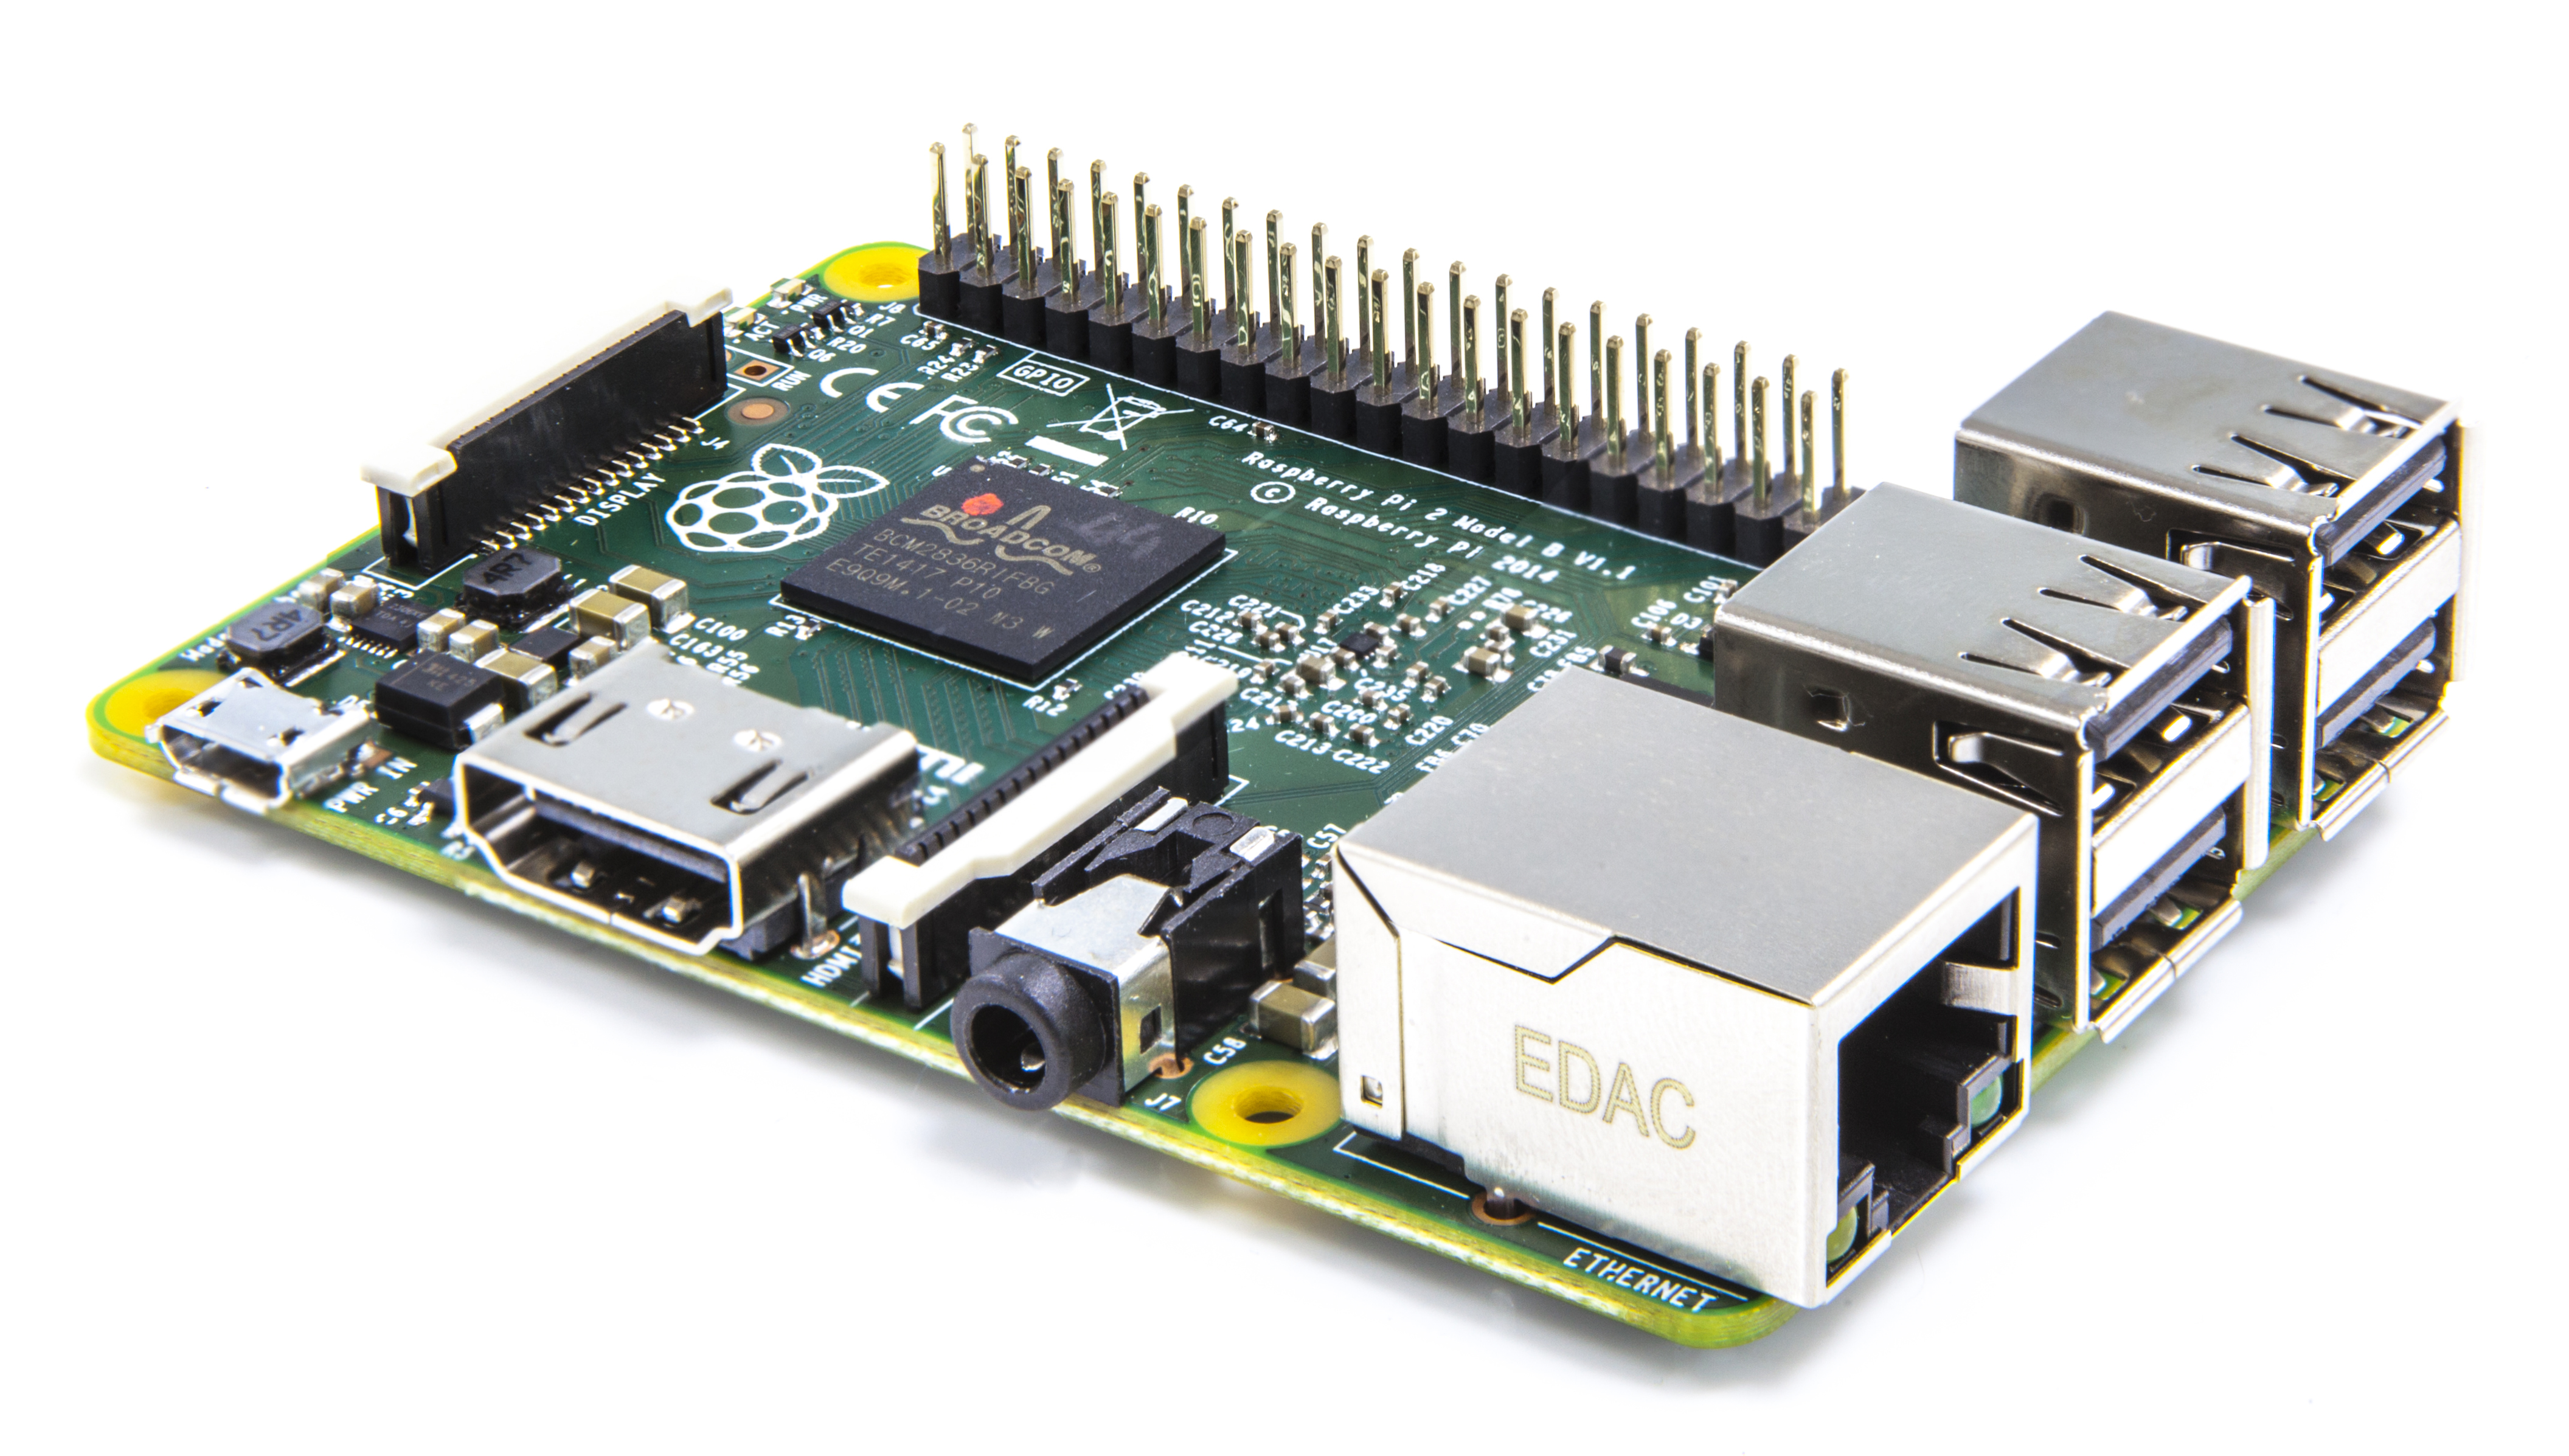
\includegraphics[width=0.3\textwidth]{./figures/rpi.jpg}
	\caption{Raspberry Pi 2 Model B. {\footnotesize Source: \url{raspberrypi.org}}}
	\label{fig:rpi}
\end{wrapfigure}
This brief analysis should be enough to prove that an SBC is more capable on almost any aspect than a microcontroller board and significantly more flexible.
Thus, for this project, a Raspberry Pi 2 Model B SBC was selected for the reasons mentioned above and additionally because it is widely available and runs a full Debian Operating System.
The only disadvantage is its higher power consumption as compared with the Arduino family of microcontrollers, which can nevertheless be neutralised by powering the OCAS with an off-the-shelf portable USB battery pack which outputs a continuous current of 5V, 2A: just enough to provide energy to the Raspberry Pi and all the peripherals.

\subsection{Other components}

Clearly, the most important components of the OCAS are its sensors and processing unit.
The other elements are less critical and the selection process was less exhaustive.
The component list considered for the prototype will only be listed here for completeness and to aid any interested researcher on the reproduction of the project.

\begin{description}
	\item[\scshape Power source] As mentioned in the previous section, any portable USB battery pack with at least 5V, 2A continuous current will sufice to power the computer board and its peripherals.
		The one used for the project is the Amazon Basics 5600 mAh battery, which can potentially last more than two hours powering the OCAS.
	\item[\scshape Network adapter] For the connection with the Ground Control Station, a wireless WiFi network will be used.
		Unfortunately, the Raspberry Pi does not include one, so the external TP-Link TL-WN822N has to be mounted on the testing platform, although any other model would be just as suitable.
	\item[\scshape Testing platform] The testing part of this project is based upon the Bachelor Thesis by M. Arteta \cite{arteta2015}, which provided an already calibrated and flight-capable F450 quadrotor UAV.
\end{description}


\begin{figure}[htbp]
	\centering
	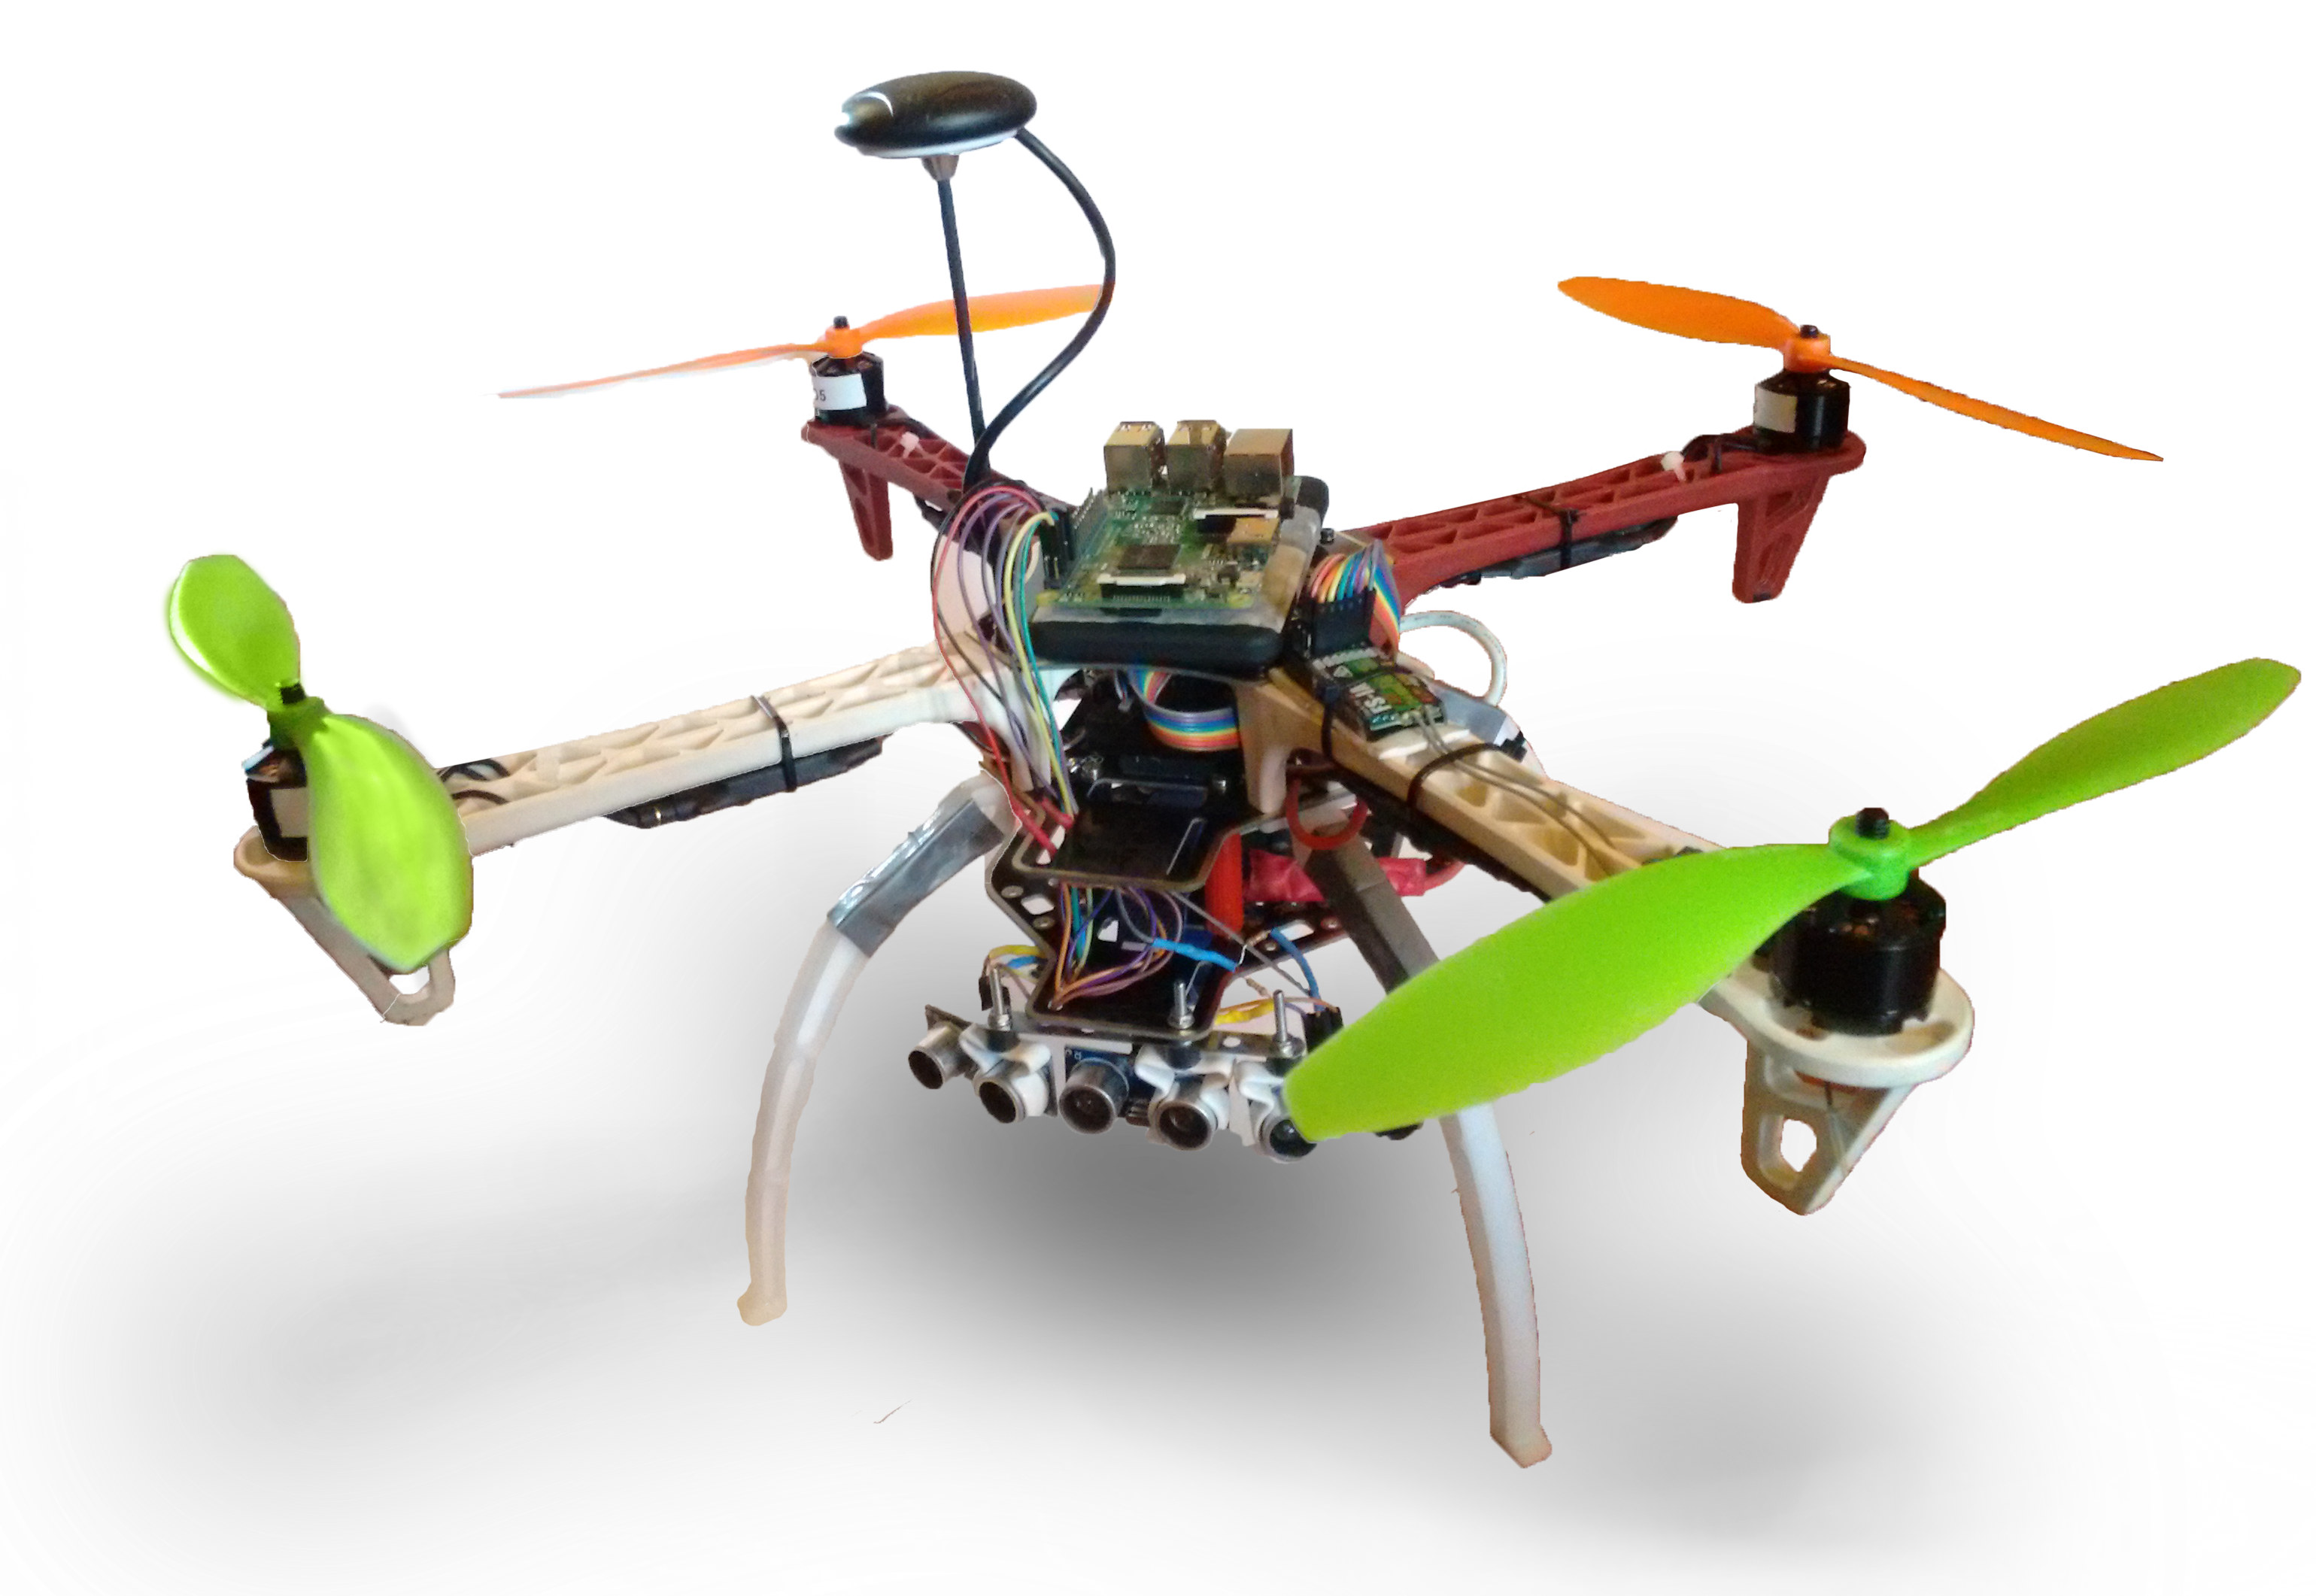
\includegraphics[width=0.6\textwidth]{./figures/platform1.png}
	\caption{Testing platform, with OCAS already integrated}
	\label{fig:platform}
\end{figure}


